\begin{frame}\frametitle{$n=\infty$}
  \begin{align*}
    r-r_{\mathrm{c}}\propto(K-K_{\mathrm{c}})^{2/3}
  \end{align*}
  \begin{figure}
    \begin{center}
      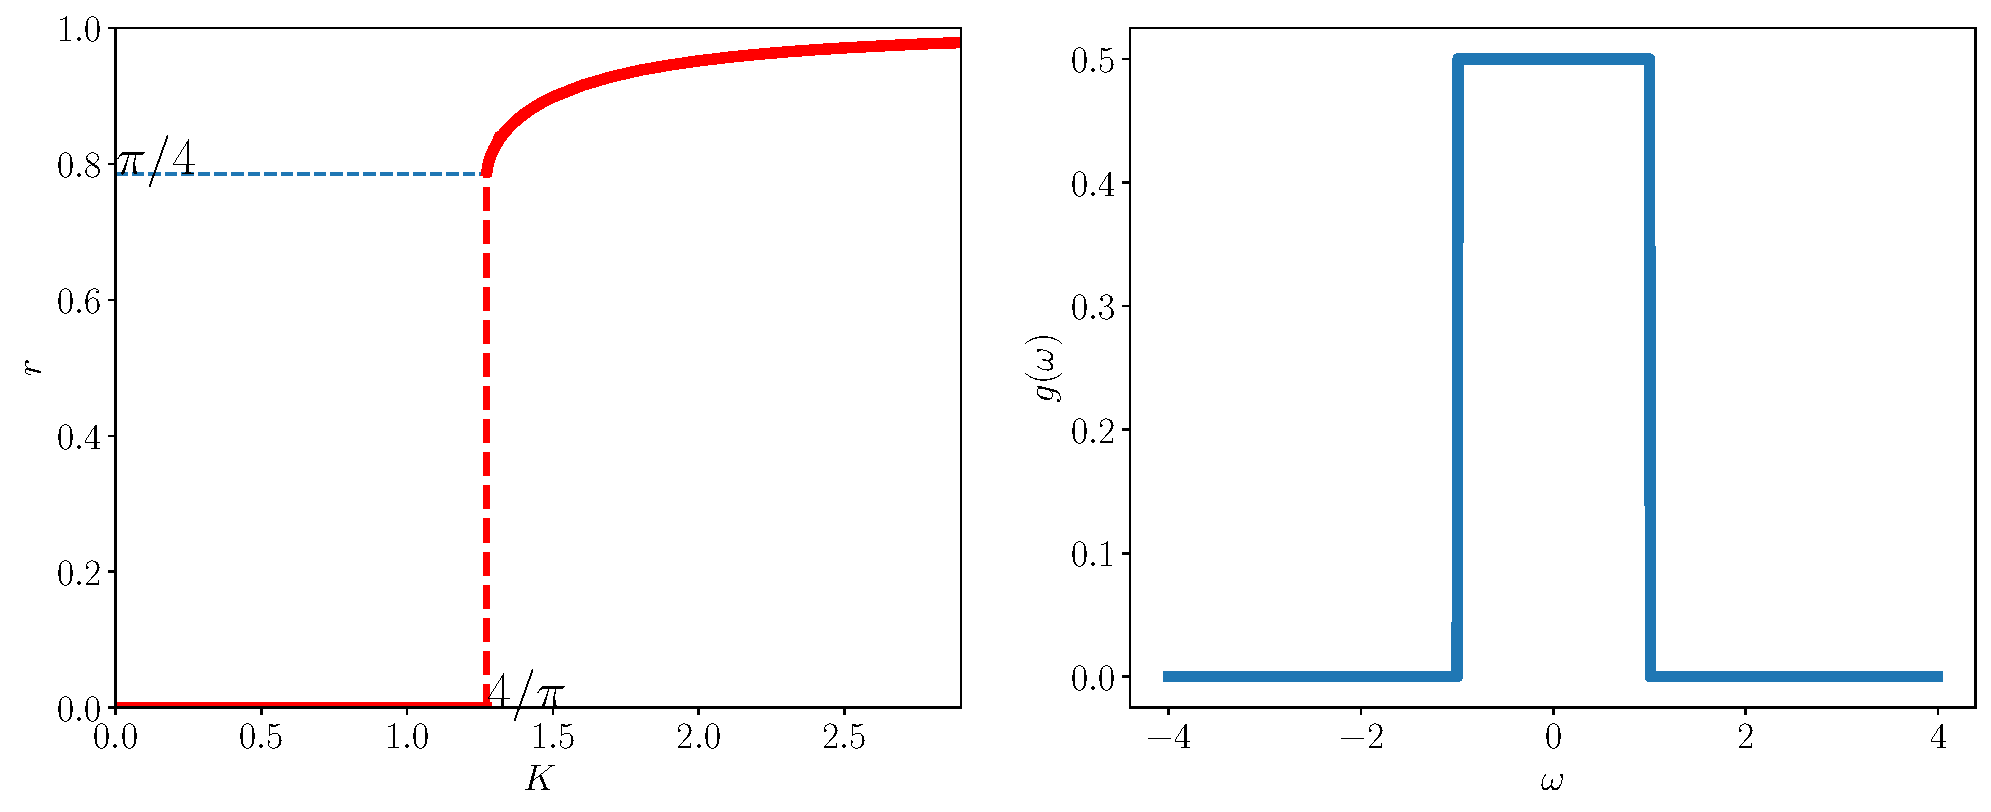
\includegraphics[scale=0.3]{figs/bif-n-inf.pdf}
    \end{center}
  \end{figure}
  \begin{itemize}
    \item 臨界点でjumpが見られる
    \item $\beta=\dfrac{2}{3}$
  \end{itemize}
\end{frame}

\begin{frame}\frametitle{$\sin2\theta$を付け加える}
  \begin{align*}
    \frac{\diff\theta_{i}}{\diff t}=\omega_{i}+\frac{K}{N}\sum_{j=1}^{N}[\sin(\theta_{j}-\theta_{i})+\blue{a\sin2(\theta_{j}-\theta_{i})}]
    \end{align*}
    \begin{figure}
    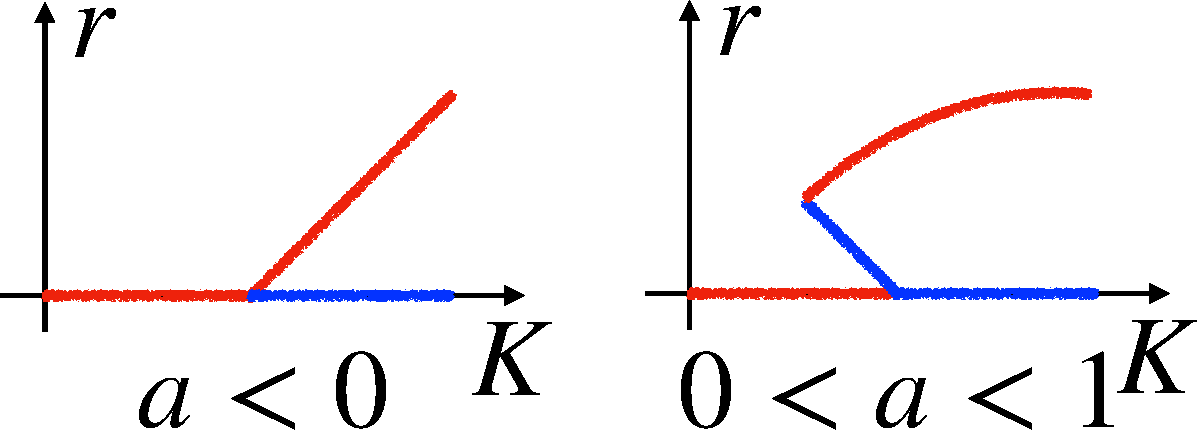
\includegraphics[scale=0.3]{figs/sin2-crop.pdf}
    \end{figure}
  \begin{itemize}
    \item \textbf{中心多様体縮約}を用いて$\beta=1$であることが示されている[Crawford 1995,Chiba 2011]。
    \begin{align*}
      &r\sim\frac{2(1-a)}{\Kc^{3}Ca}(K-\Kc)^{\red{1}}+\cdots\\
      &C=\mathcal{PV}\int_{\mathbb{R}}\diff\omega\frac{g'(\omega)}{\omega}
    \end{align*}
  \end{itemize}
\end{frame}

\begin{frame}\frametitle{Watts--Strogatz model}
\begin{block}{アルゴリズム}
  \begin{itemize}
    \item[1] $N$個の頂点を持つ$k$-隣接グラフを生成する。
    \item[2] $kN$本の枝のそれぞれに対して、確率$p$でエッジの一方(ランダムに選ぶ)の結合を切り離し、$N$頂点の中からランダムに選ばれた頂点につなぎ替える。
    ただし、自己ループや多重エッジができないようにする。 
  \end{itemize}
\end{block}
\begin{figure}
  \begin{center}
    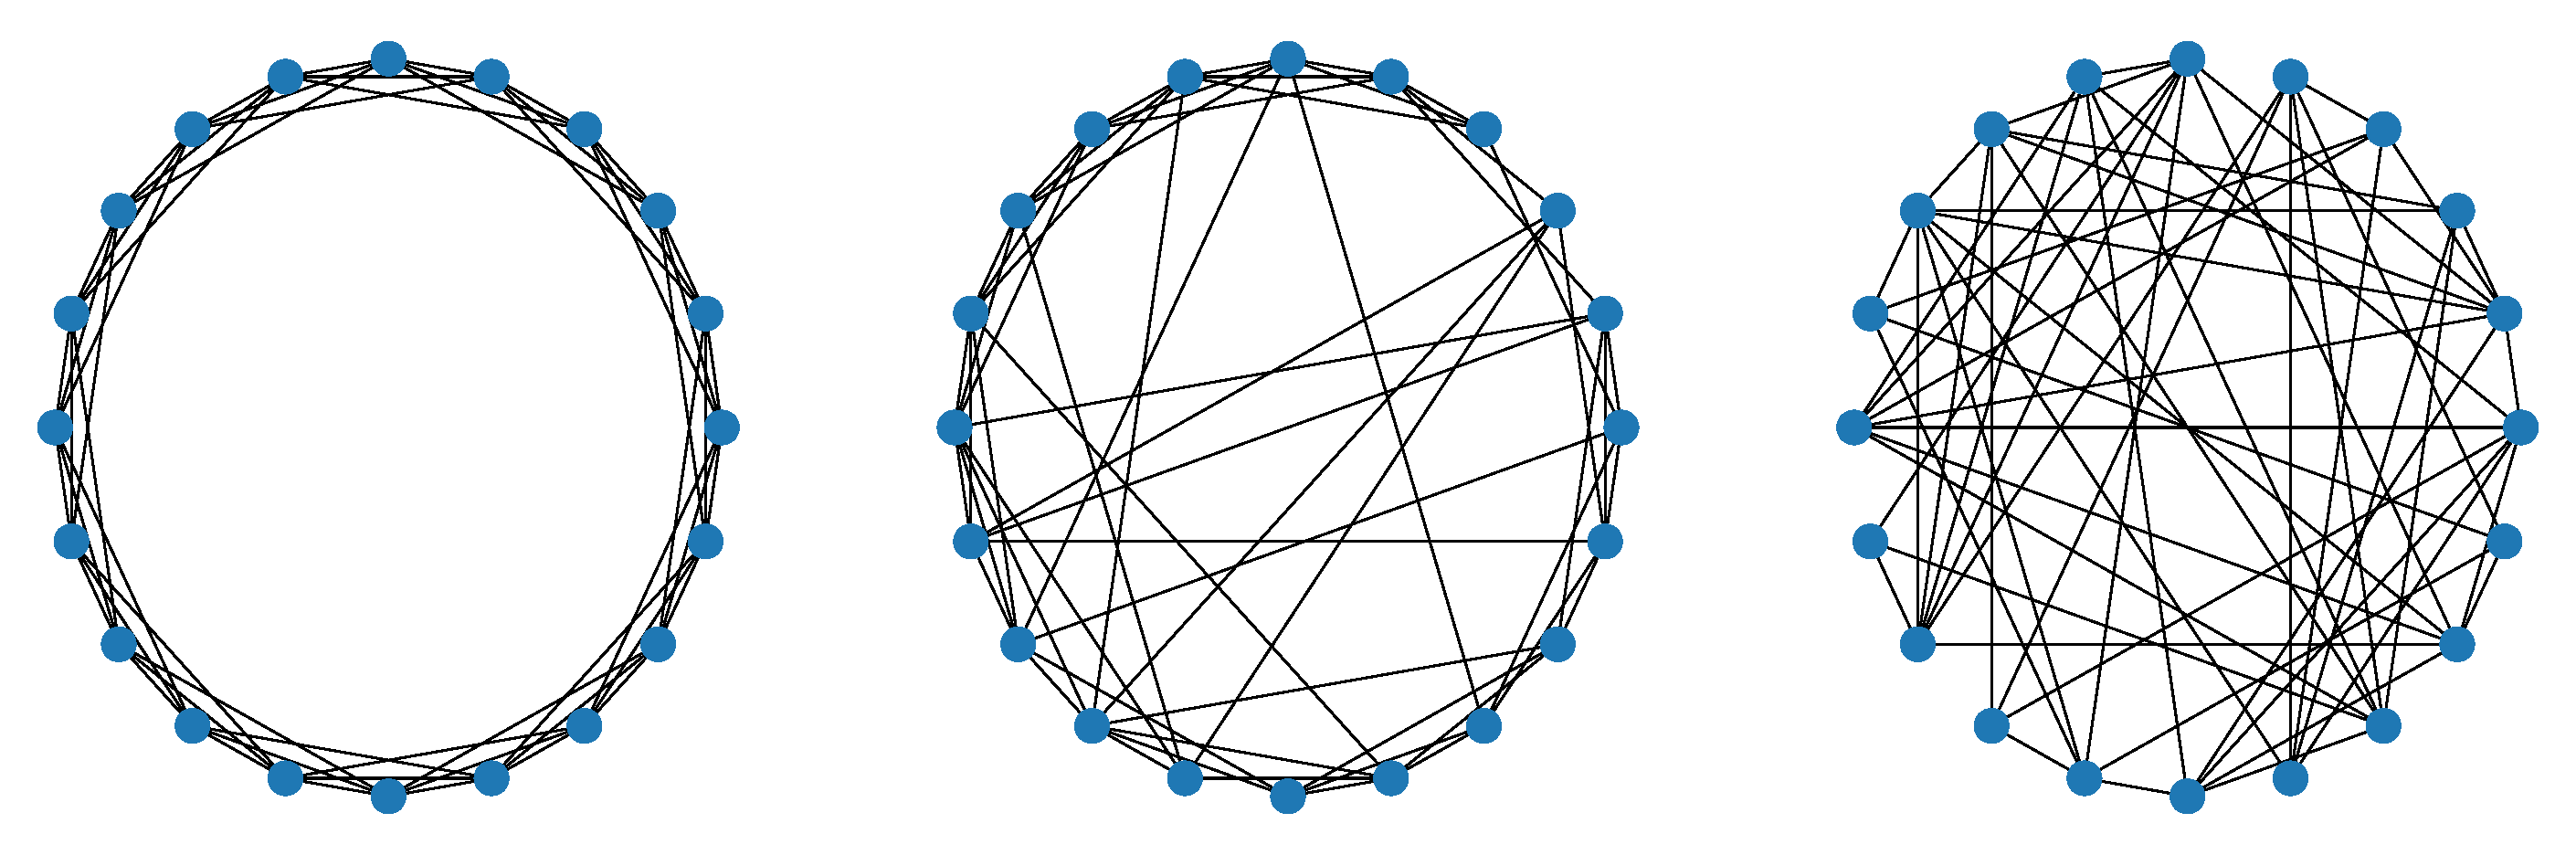
\includegraphics[width=11cm]{figs/ring_sw.pdf}
  \end{center}
\end{figure}
\end{frame}

\begin{frame}\frametitle{$O(N^{2})$ small-worldとの違い}
  [Chiba et al. 2018]の中でスモールワールドネットワーク上の蔵本モデルの計算をしているが、
  彼らは$k=\lfloor rN\rfloor, r\in(0,0.5)$としている。
  \begin{figure}
    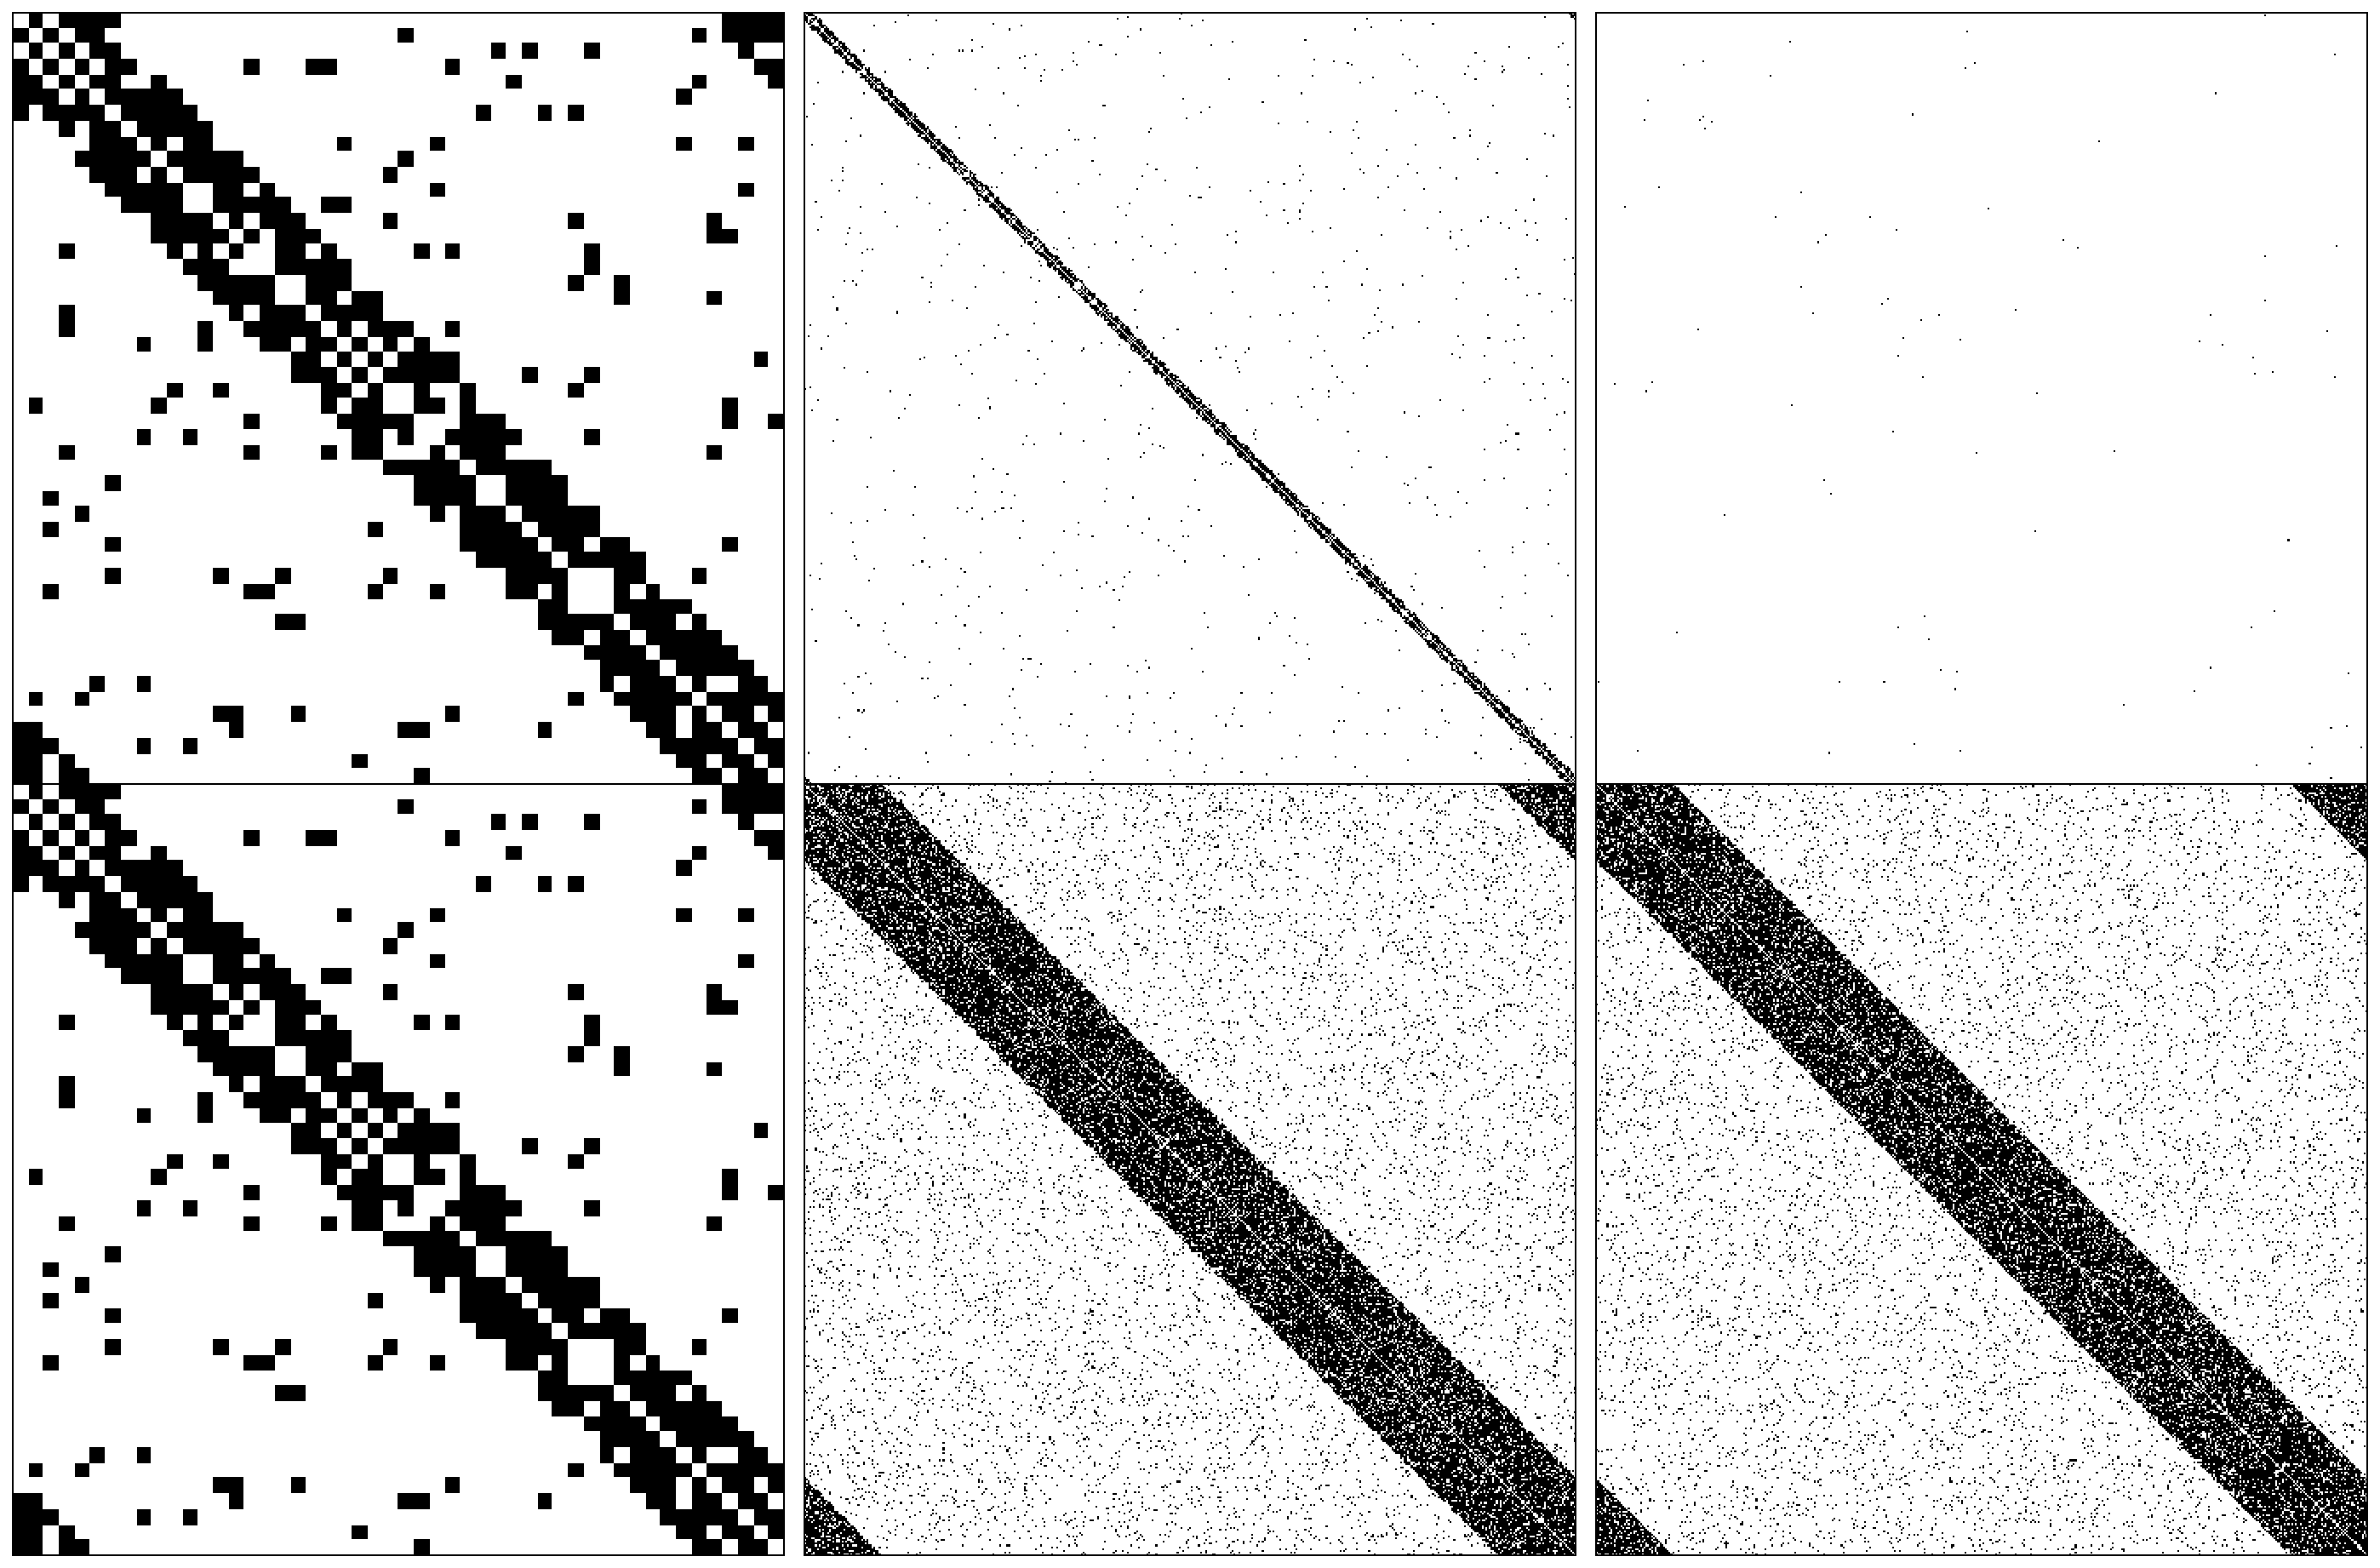
\includegraphics[scale=0.15]{figs/graphon.pdf}
  \end{figure}
  \begin{itemize}
    \item $r$の立ち上がりが
    \begin{align*}
      r\sim\frac{C}{\sqrt{-g''(0)}}(K-\Kc)^{1/2}+\cdots
    \end{align*}
    \item この設定だと$\beta$が$g(\omega)$に依存することを示唆している。(全結合と変わらない結果になりうる。)
  \end{itemize}
\end{frame}

\begin{frame}\frametitle{$a=0.5$}
  \begin{itemize}
    \item $a=0.5$ではヒステリシスが起こることが確認された。
    \item 不連続転移(1次相転移)が起こることを示唆している。
    \item $(a,n)=(0.5,1)$でシステムサイズ$N=25600$におけるヒステリシス
    \begin{figure}
      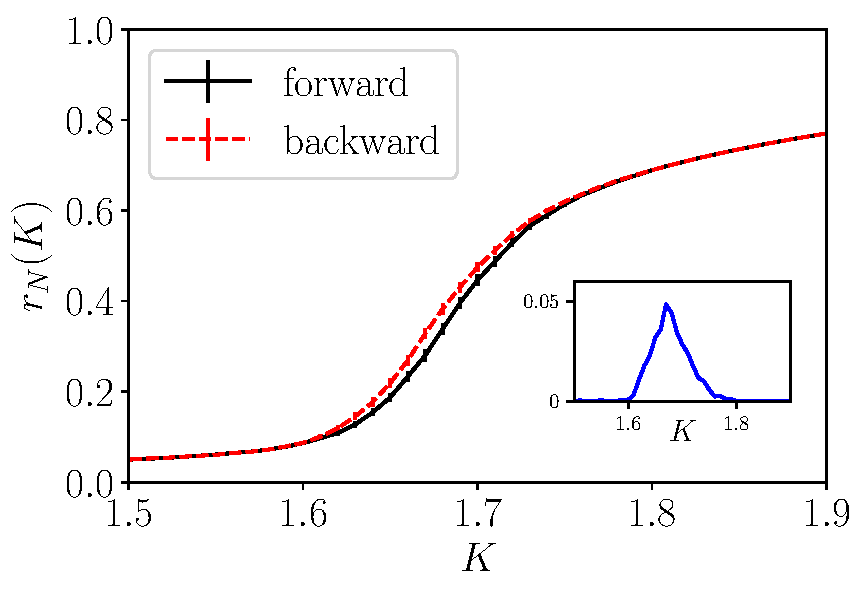
\includegraphics[width=9cm]{figs/hysteresis.pdf}
    \end{figure}
  \end{itemize}
\end{frame}

\begin{frame}{$\mu^{(N,p)}$の数値計算}
\begin{itemize}
    \item 最適化ライブラリ: \texttt{JuMP}(\texttt{Julia}), \texttt{pulp}(\texttt{Python})
\end{itemize}
\begin{figure}
    \centering
    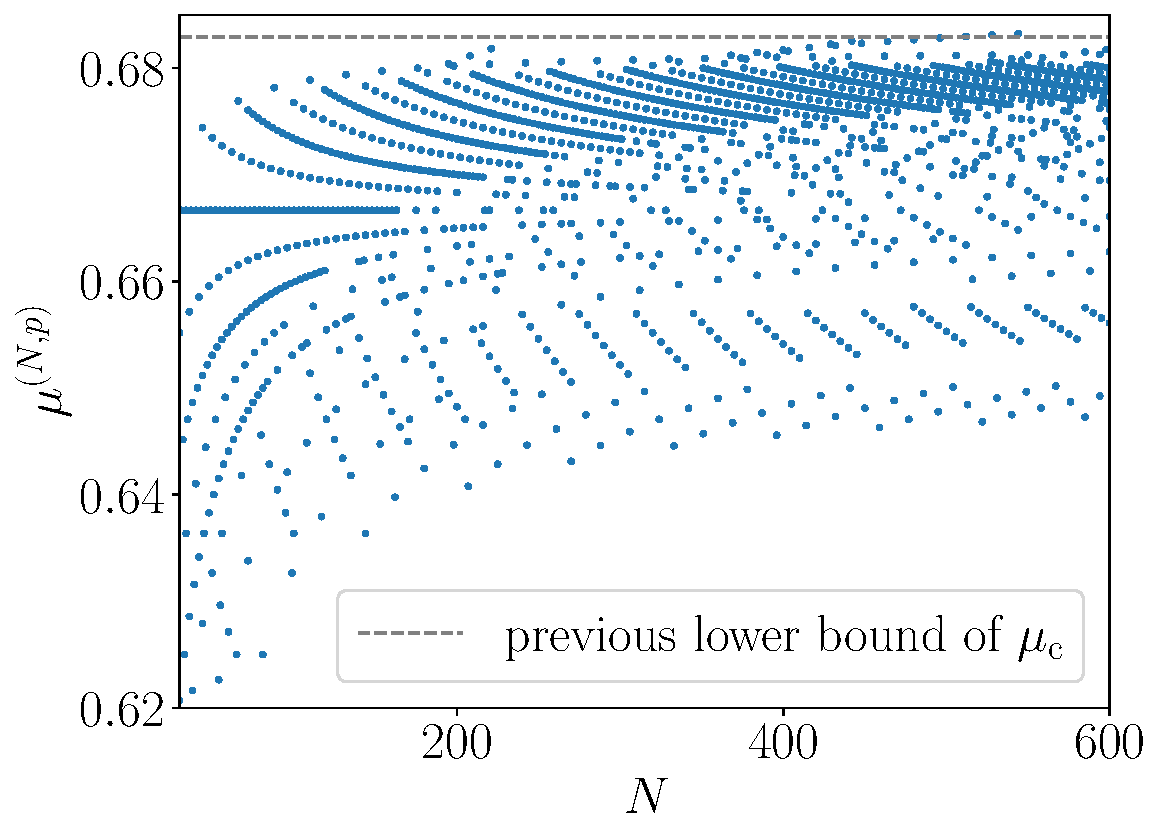
\includegraphics[width=0.9\textwidth]{figs/max_connect.pdf}
\end{figure}
\end{frame}

\begin{frame}{ネットワーク密度}
    \begin{block}{ネットワーク密度$d$}
        \[
            d = \frac{\sum_{i,j\in[N]}a_{ij}}{N(N-1)}
        \]
    \end{block}
    \begin{itemize}
        \item 可能なすべての辺の数に対する辺の数の比
        \item 全結合ネットワークで$d=1$
        \item $d$が大きいからといって同期するわけではない
    \end{itemize}
    \begin{figure}
        \begin{center}
            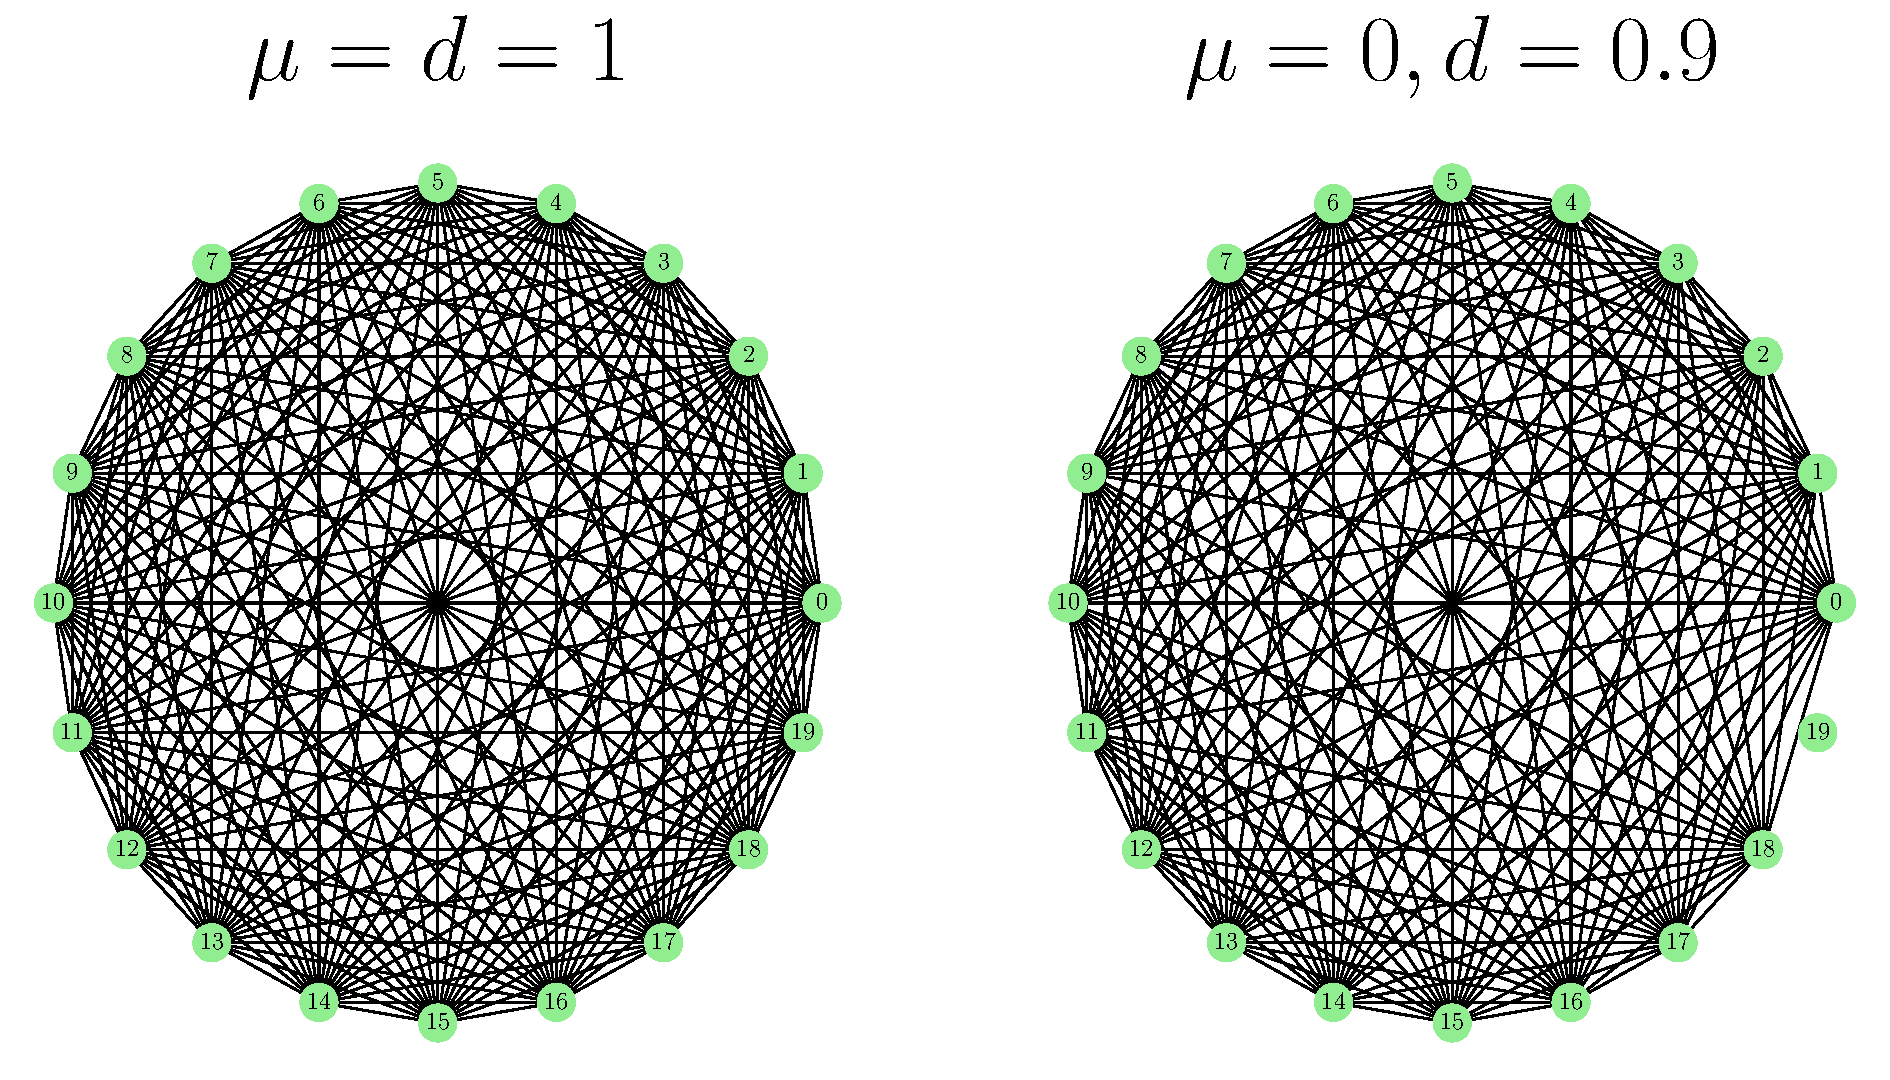
\includegraphics[width=0.6\textwidth]{figs/density.pdf}
        \end{center}
    \end{figure}
\end{frame}

\begin{frame}{巡回行列}
\begin{itemize}
\item $\bm{x}\in \mathbb{R}^{N}$から生成される巡回行列$A\in\mathbb{R}^{N\times N}$
\begin{align*}
A &= \left(a_{ij}\right)_{1\leq i,j\leq N}=\left(x_{j-i}\right)_{1\leq i,j\leq N}\notag\\
&=
\begin{pmatrix}
    x_{0} & x_{1} & \dots & x_{N-2} & x_{N-1}\\
    x_{N-1} & x_{0} & x_{1} &  & x_{N-2}\\
    \vdots & x_{N-1} & x_{0} & \ddots & \vdots\\
    x_{2} &  & \ddots & \ddots & x_{1}\\
    x_{1} & x_{2} & \dots & x_{N-1} & x_{0}
\end{pmatrix}
\end{align*}
\item 行列$A$の固有値$\lambda_{k},k=0,1,\dots,N-1$
\begin{align*}
\lambda_{k}=\sum_{l=0}^{N-1}x_{l}\exp\left(\frac{2\pi ikl}{N}\right)
\end{align*}
\end{itemize}
\end{frame}

\begin{frame}{$(N,p)=(19m,m)$}
\begin{figure}
    \begin{center}
        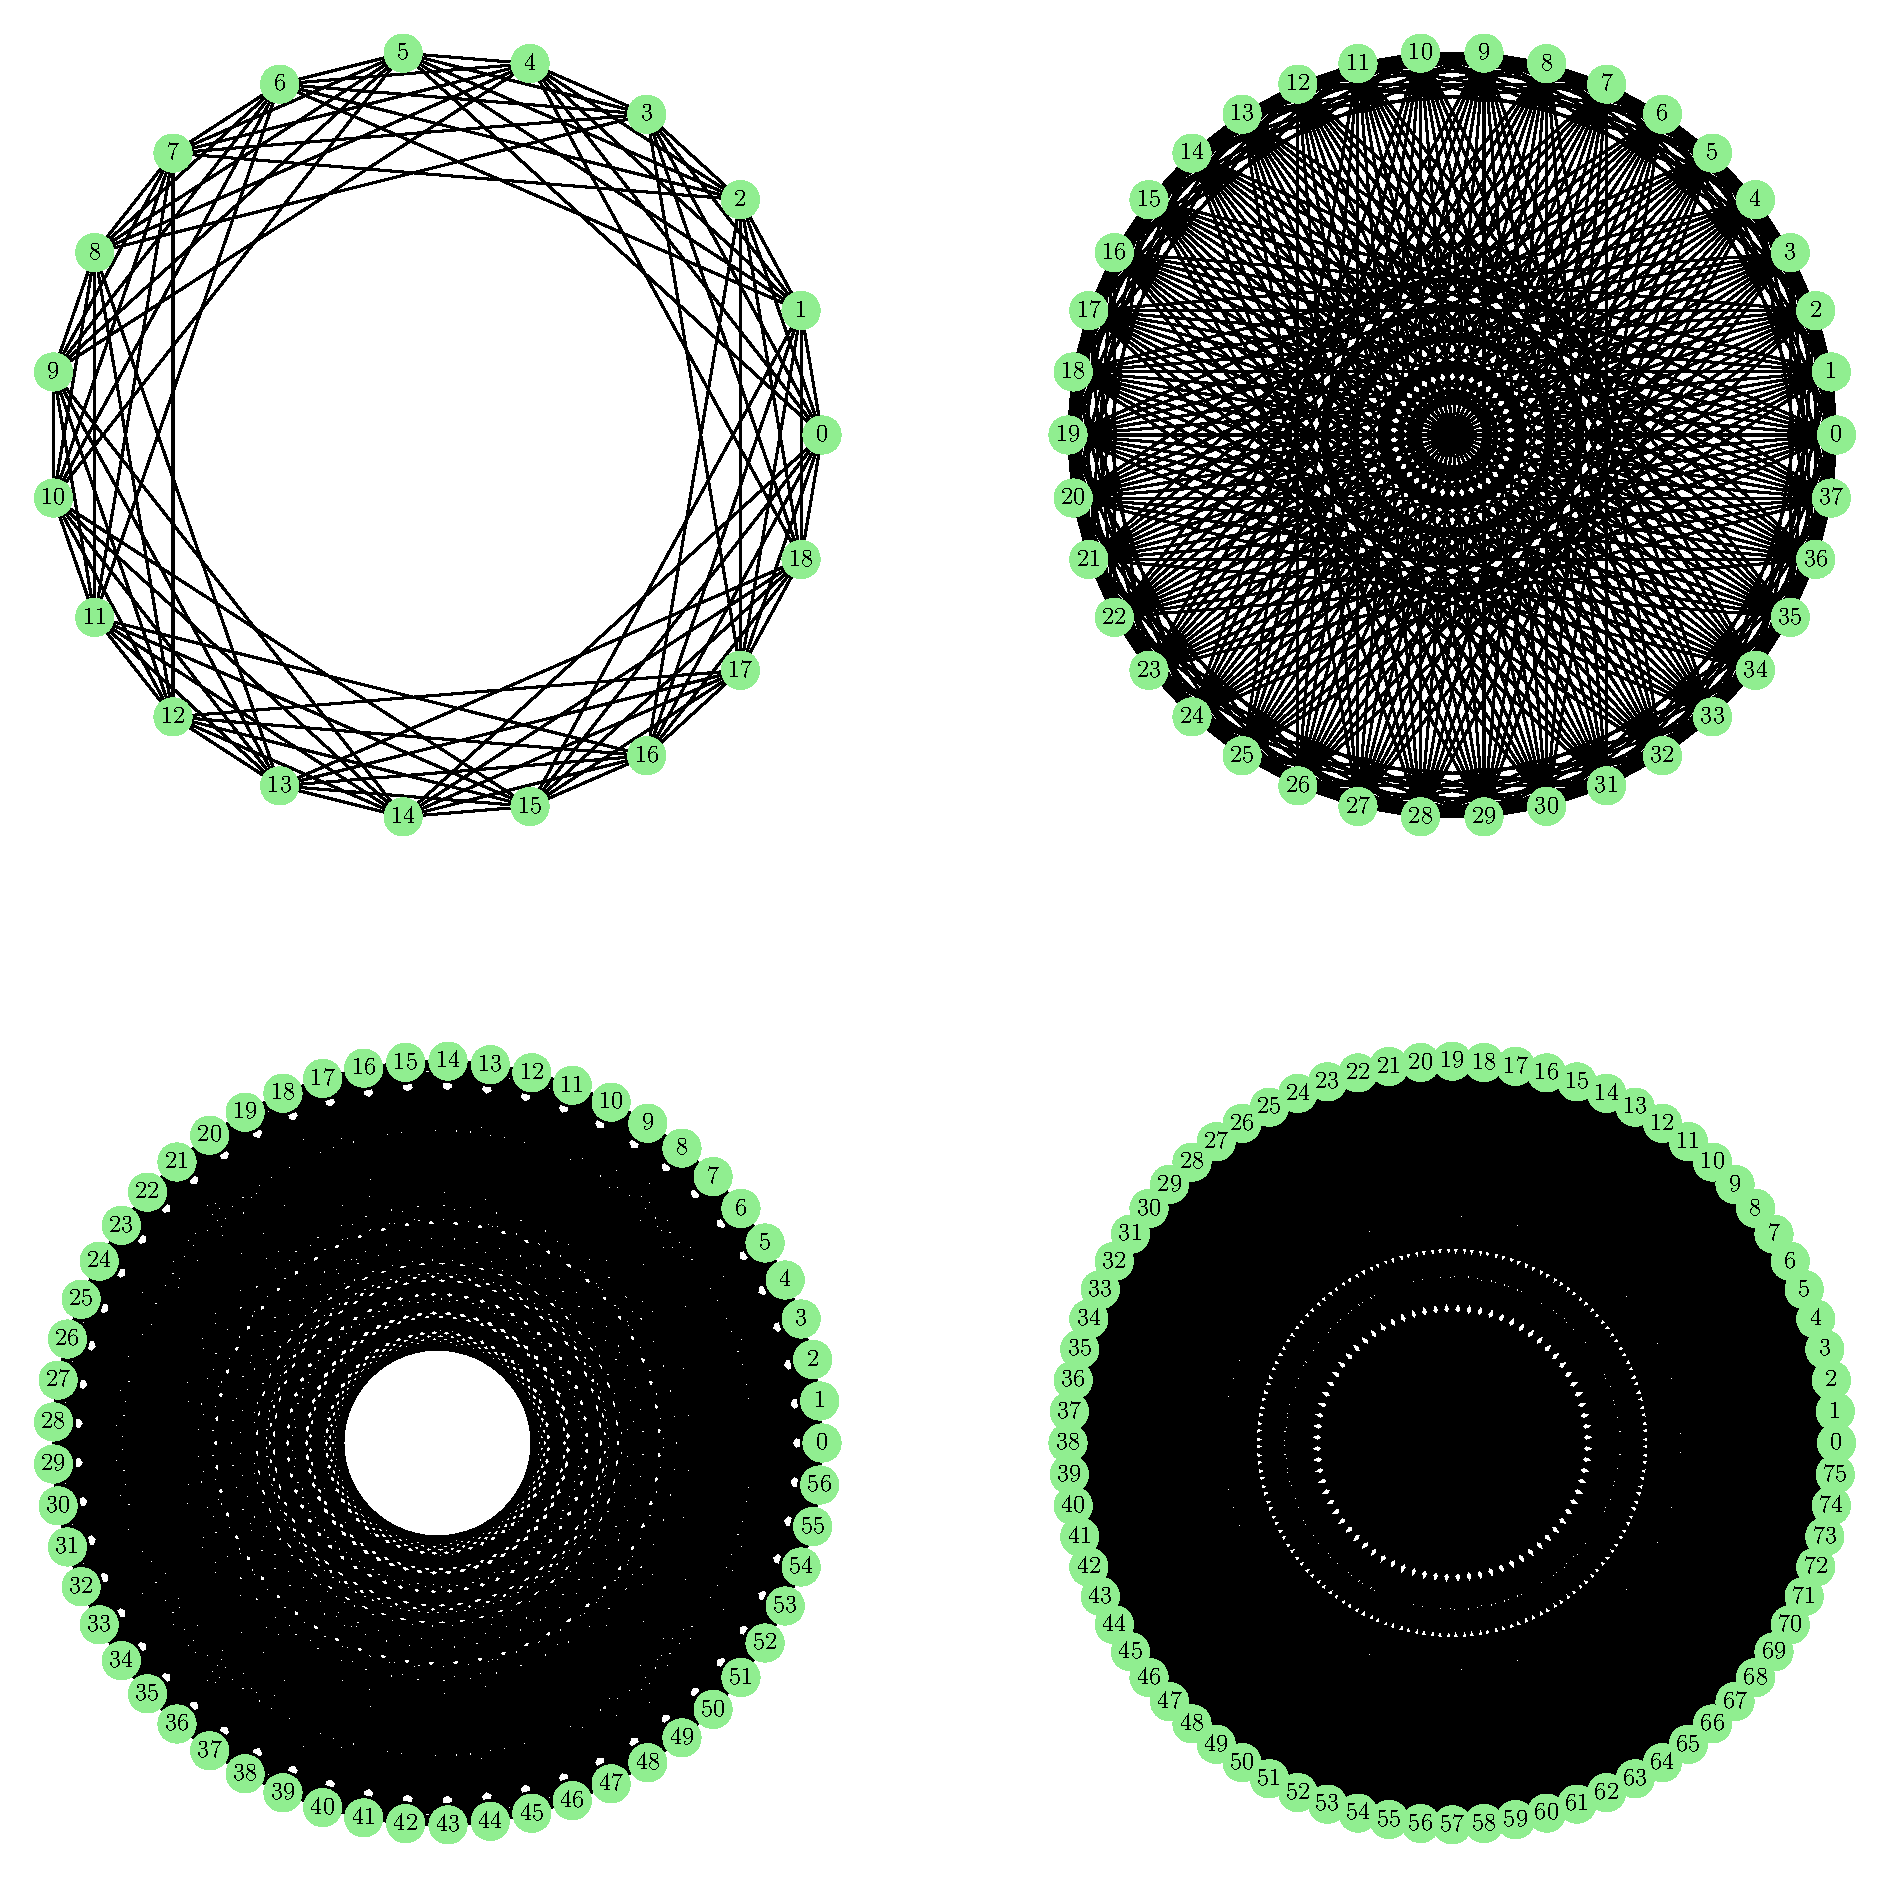
\includegraphics[width=0.65\textwidth]{figs/19.pdf}
    \end{center}
\end{figure}
\end{frame}

\begin{frame}{大規模データに対する処方箋}

  \begin{itemize}
    \item \textbf{補助変数法(sparse GP)}\footnote{Quiñonero-Candela 2005}
    \begin{itemize}
      \item $m(<n)$個の補助入力点を用いて計算を効率化
    \end{itemize}
    \item \textbf{変分ベイズ法(SVGP)}\footnote{Hensman 2013}
    \begin{itemize}
      \item $m(<n)$個の補助入力点を用意
      \item 変分事後分布を学習し真の事後分布に近似
      \item データをサイズ$b$のミニバッチにわけることで学習を効率化
    \end{itemize}
  \end{itemize}
  
  \begin{table}[H]
    \caption*{計算量の比較}
    \begin{tabular}{l|cc>{\columncolor[rgb]{1.0,1.0,0.7}}c}
      & GP & sparse GP & SVGP \\\hline\hline
     推論コスト & $\mathcal{O}(n^{3})$ & $\mathcal{O}(nm^{2})$ & $\mathcal{O}(bm^{2}+m^{3})$ \\
     メモリコスト & $\mathcal{O}(n^{2})$ & $\mathcal{O}(nm)$ & $\mathcal{O}(bm+m^{2})$ \\
    \end{tabular}
  \end{table}
  
  \begin{itemize}
    \item 本研究ではSVGPを用いる
  \end{itemize}
\end{frame}


\begin{frame}{ベイズ線形回帰との比較}
  適切な次数の選択に失敗している
  \begin{figure}
    \centering
    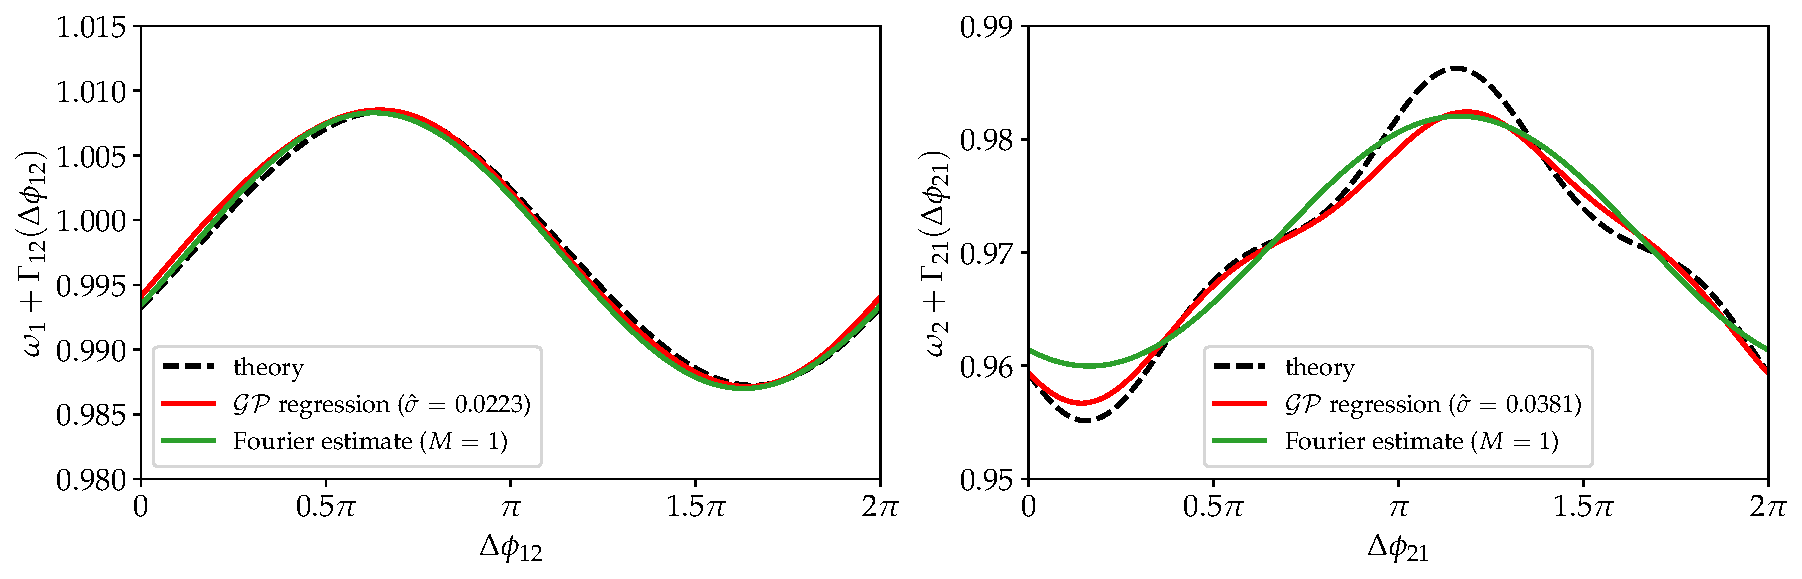
\includegraphics[width=\textwidth]{figs/vdp.pdf}
  \end{figure}
  \begin{figure}
    \centering
    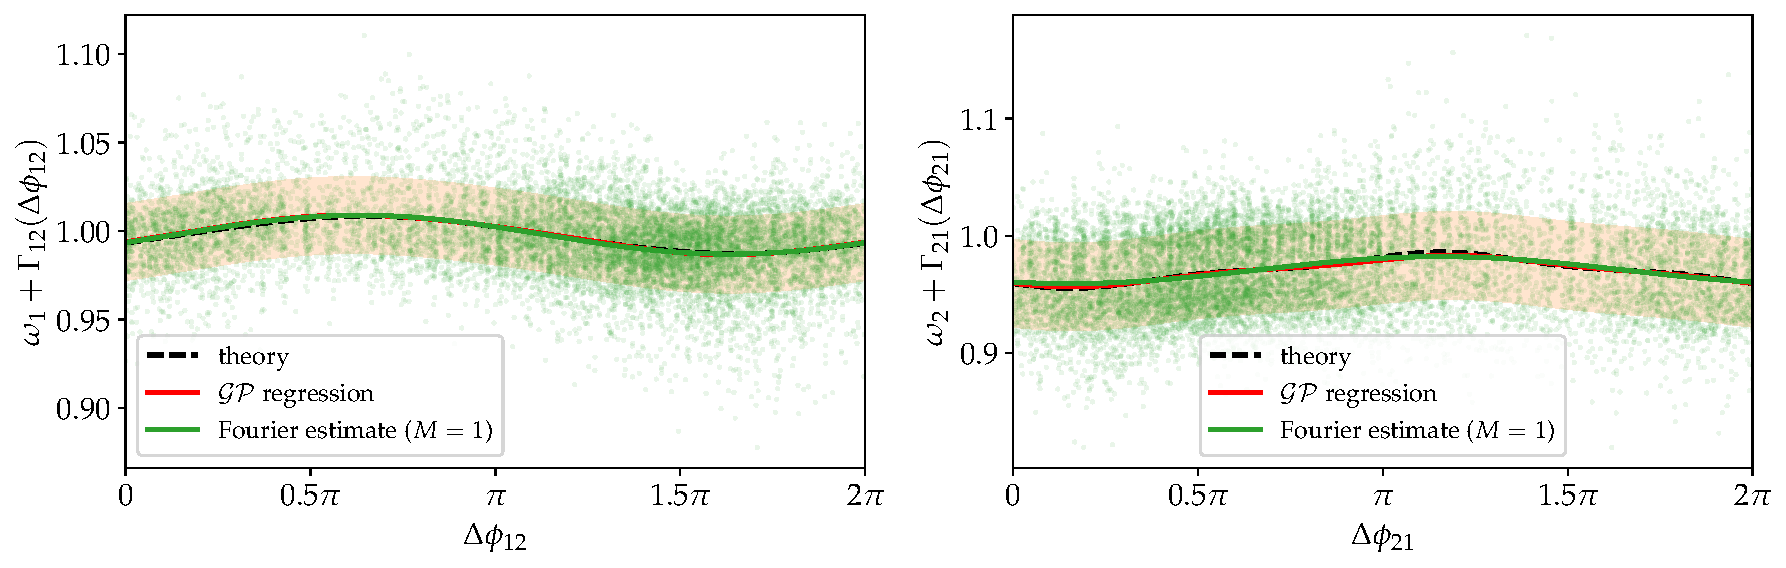
\includegraphics[width=\textwidth]{code/vdp_20221121/fig20221121/exp01case01_errorbar.pdf}
  \end{figure}
\end{frame}